\chapter{Практические задания}

Что получится при вычисления каждого из выражений?
\begin{figure}[ht!]
	\centering{
		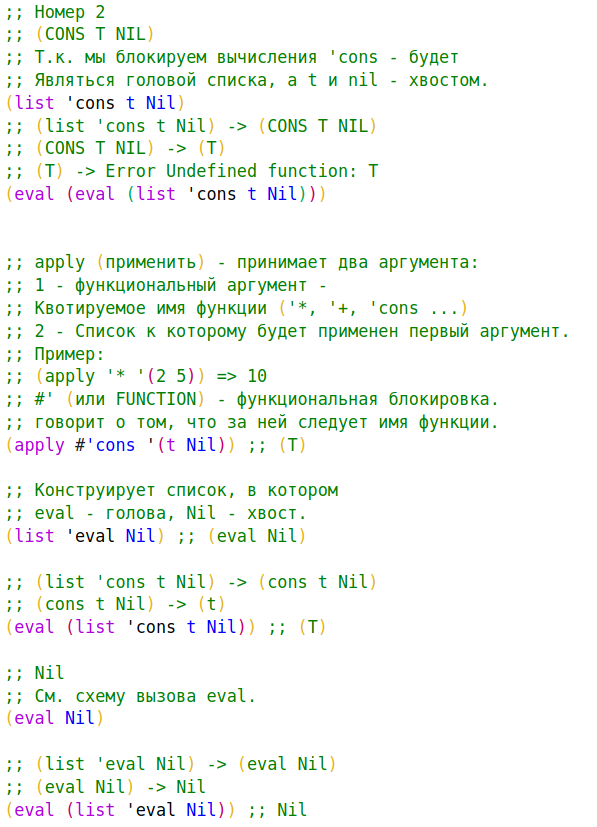
\includegraphics[width=1\textwidth]{img/2.png}
		\caption{Задание 2} }
\end{figure}

Написать функцию, которая переводит температуру в системе Фаренгейта температуру по Цельсию.
\begin{figure}[ht!]
	\centering{
		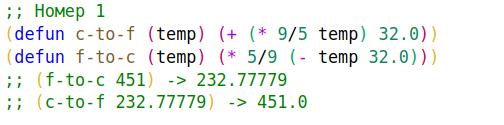
\includegraphics[width=1\textwidth]{img/1.png}
		\caption{Задание 1} }
\end{figure}

\begin{enumerate}
	\item Доп 1. Написать функцию, вычисляющую катет по заданной гипотенузе и другому катету прямоугольного треугольника.
	\item Доп 2. Написать функцию, вычисляющую площадь трапеции по ее основаниям и высоте.
\end{enumerate}

\begin{figure}[ht!]
	\centering{
		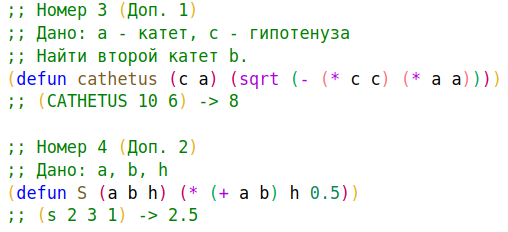
\includegraphics[width=1\textwidth]{img/3.png}
		\caption{Задание 3} }
\end{figure}


\chapter{Ответы на вопросы}

\section{Синтаксическая форма и хранение программы в памяти}

В Lisp формы представления программы и обрабатываемых ею данных 
представляется в виде S-выражения. В памяти представляется как атом 
(5 указателей) или точечная пара (бинарный узел, 2 указателя)

\section{Трактовка элементов списка}

Первый элемент списка - это имя функции, остальные аргументы.

\section{Порядок реализации программы}

Интерпретатор ожидает ввода S-выражения, после чего предает 
введенное S-выражение функции eval и выводит полученый результат.

\begin{figure}[ht!]
	\centering{
		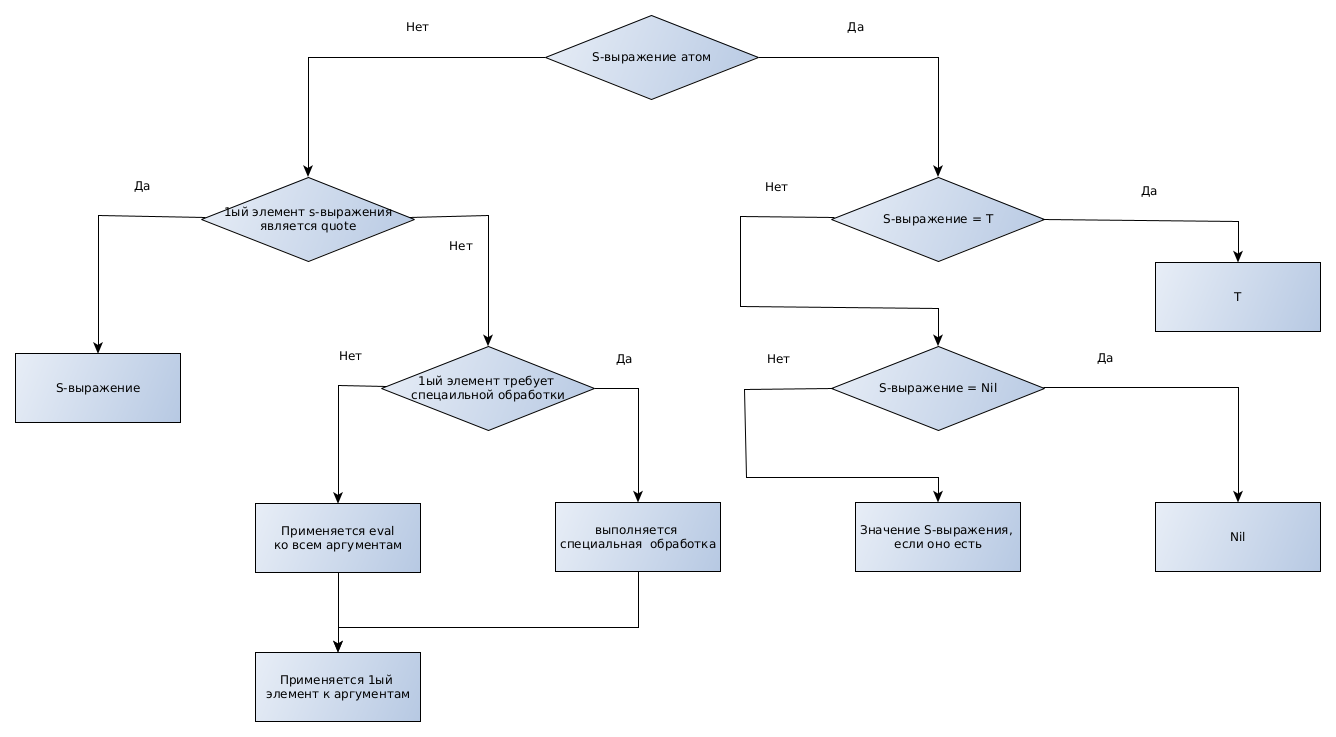
\includegraphics[width=1\textwidth]{img/eval.png}
		\caption{Схема работы функции eval} }
\end{figure}

\section{Способ определения функции}

1. С помощью lambda. 

Базовое определение лямбда-выражения:

\begin{lstlisting}[language=Lisp]
	(lambda лямбда-список тело_функции)
\end{lstlisting}

Пример:

\begin{lstlisting}[language=Lisp]
	(lambda (x y) (+ x y))
\end{lstlisting}

Применение лямбда-выражений:

\begin{lstlisting}[language=Lisp]
	(лямбда-выражение фактические_параметры)
\end{lstlisting}

Пример:

\begin{lstlisting}[language=Lisp]
	((lambda (x y) (+ x y)) 1 2) ;; 3
\end{lstlisting}

2. С помощью defun. 
Для неоднократного применения функции (а также для построения
рекурсивной функции) используется встроенная функция defun.

Синтаксис:

\begin{lstlisting}[language=Lisp]
	(defun имя_функции лямбда-список тело_функции)
\end{lstlisting}

Пример:

\begin{lstlisting}[language=Lisp]
	(defun sum (x y) (+ x y))
\end{lstlisting}

Пример вызова:

\begin{lstlisting}[language=Lisp]
	(sum 1 2) ;; 3
\end{lstlisting}


